\documentclass[a4paper]{article}
\usepackage[affil-it]{authblk}

\usepackage[UTF8]{ctex}
\usepackage{amsmath}
\usepackage{amssymb}
\usepackage{geometry}
\usepackage{graphicx}

\geometry{margin=1.5cm, vmargin={0pt,1cm}}
\setlength{\topmargin}{-1cm}
\setlength{\paperheight}{29.7cm}
\setlength{\textheight}{25.3cm}

\newcommand{\esm}{\epsilon_M}
\newcommand{\fl}{\text{fl}}
\newcommand{\Eabs}{E_{\text{abs}}}
\newcommand{\Erel}{E_{\text{rel}}}
\newcommand{\abs}[1]{\left|#1\right|}
\newcommand{\normtwo}[1]{\left\|#1\right\|_2}
\newcommand{\norminf}[1]{\left\|#1\right\|_{\infty}}
\newcommand{\norm}[1]{\left\|#1\right\|}
\begin{document}
% =================================================
\title{Numerical Analysis homework \# 3}

\author{梁育玮 Liang Yuwei 3230102923
  \thanks{Electronic address: \texttt{liangyuwei631@gmail.com}}}
\affil{(Mathematics and Applied Mathematics 2302), Zhejiang University }
\date{\today}

\maketitle


% ============================================
\section{Assignment}
\subsection*{I. Convert 477 to binary.}
we have $477 = 2^8 + 2^7 + 2^6 + 2^2 + 2^0 = (111011101)_2$. Thus in FPN, $477 = (1.11011101)_2 \times 2^8$.

\subsection*{II. Convert $\frac{5}{3}$ to binary.}
\begin{align*} 
  \frac{3}{5} &= (0.\dot{1}00\dot{1})_2 \\
  &= (1.\dot{0}01\dot{1} )_2 \times 2^0
\end{align*}

\subsection*{III. Prove $x_R - x = \beta(x - x_L)$}
denote $\alpha = \beta -1$, which is the biggest digit in the FPN. Then we have
\[x_L = (\alpha.\alpha\alpha\ldots\alpha\alpha)_{\beta} \times \beta^{e-1},\quad x_R = (1.00\ldots 01)_{\beta} \times \beta^{e} .\]

Thus we have
\[x - x_L = \epsilon_M \beta^{e-1},\quad x_R - x = \epsilon_M \beta^{e}.\]

Therefore, $x_R - x = \beta(x - x_L)$.

\subsection*{IV. Two normalized FPNs adjacent to $x = \frac{5}{3}$}
The two normalized FPNs adjacent to $x = \frac{5}{3}$ are $x_L = (1.1010\dots101)_2 \times 2^0$ and $x_R = (1.1010\dots110)_2 \times 2^0$. 
Thus we have \begin{align*}
  x - x_L &= \epsilon_M (\frac{1}{4} + \frac{1}{16} + \frac{1}{64} + \dots)\\
&= \esm \frac{\frac{1}{4}}{1-\frac{1}{4}} = \frac{1}{3} \esm,\\
  x_R - x_L &= \esm\\
  \implies x_R - x &= \frac{2}{3} \esm.
\end{align*}  
Thus we have $x - x_L \le x_R -x$, which means $\fl(x) = x_L$.

Moreover, we have 
\[\Eabs(\fl(x)) = x- x_L = \frac{\esm}{3} = \frac{1}{3\times 2^{23}}\]

\subsection*{V. Unit roundoff}
Let $x$ be a float close to $1 + \esm$. As $x$ approaches $1 + \esm$ from the left, $fl(x) = 1$, and we have:
\[\Erel(\fl(x)) = \frac{x-1}{x} = \frac{\esm}{1 + \esm} \approx \esm\]
So the unit roundoff is $\esm$.

\subsection*{VI. Substraction $1 - \cos x$ when $x = \frac{1}{4}$}
We assume the opration is under the FPN system single precision.

$\cos \frac{1}{4} = (1.111 1000 0000 1010 1010 0101)_2 \times 2^{-1}$
\begin{align*}
  1 - \cos \frac{1}{4} &= (1.000 0000 0000 0000 0000 0000)_2 \times 2^0 - (1.111 1000 0000 1010 1010 0101)_2 \times 2^{-1}\\
&= (1.000 0000 0000 0000 0000 0000)_2 \times 2^0 - (0.1111 1000 0000 1010 1010 0101)_2 \times 2^{0}\\
&=(1.110 0000 1010 1011 1111 1110) \times 2^{-7}.
\end{align*}

so 7 bits of precision are lost.

\subsection*{VII. Avoid catastrophic cancellation}
there are two ways to avoid catastrophic cancellation:
\subsubsection*{Taylor series}
\[  1 - \cos x = \frac{x^2}{2} - \frac{x^4}{4!} + \frac{x^6}{6!} + \dots\]

\subsubsection*{Use trigonometric identity}
\begin{align*}
  1- \cos x &=  2\sin^2\frac{x}{2}\\
&= 2\left(\frac{x}{2} - \frac{x^3}{48} + \frac{x^5}{3840} + \dots\right)^2
\end{align*}

\subsection*{VIII. condition number}
\subsubsection*{(1) $f = (x-1)^\alpha$}
The condition number is
\[
  C_f(x) = \abs{\frac{\alpha x}{x-1}}
\]
And when $x$ is close to 1, $C_f(x)$ is large.

\subsubsection*{(2) $f = \ln x$}
The condition number is
\[
  C_f(x) = \frac{1}{\abs{\ln x}}
\]
And when $x$ is close to 1, $C_f(x)$ is large.

\subsubsection*{(3) $f = e^x$}
The condition number is
\[
  C_f(x) = \abs{x}
\]
And when the absolute value of $x$ is large, $C_f(x)$ is large.

\subsubsection*{(4) $f = \arccos {x}$}
The condition number is
\[
  C_f(x) = \abs{\frac{x}{\sqrt{1-x^2}\arccos {x}}}
\]
And when $x$ is close to 1 or -1, $C_f(x)$ is large.

\subsection*{IX. Consider the function $f(x) = 1-e^{-x}$ for $x\in [0,1]$}
\subsubsection*{IX-a}
The condition number is\[ 
\text{cond}_f(x) = \abs{\frac{xe^{-x}}{1-e^{-x}}} = \frac{x}{e^{x} - 1}.
\]

Then, we need to show $x \leq e^x - 1$ for $x \in [0,1]$, which is trival. Thus we have $\text{cond}_f(x) \leq 1$.

\subsubsection*{IX-b}
Assume there exists $x_A$ such that \[
1-e^{-x_A} = (1-e^{-x})(1+\delta).  \]

Then we have \[
\delta = \frac{e^{-x} - e^{-x_A}}{1-e^{-x}} = \frac{1 - e^{x-x_A}}{e^{x} - 1} \approx \frac{x_A - x}{e^x - 1}.\]

Therefore, The condition number for algorithm $A$ is \begin{align*}
  \text{cond}_A(x) &= \frac{1}{\epsilon_u}\abs{\frac{x_A-x}{x}}\\
&= \frac{1}{\epsilon_u}\frac{\delta(e^x-1)}{x} \\&\leq \frac{e^x-1}{x}
\end{align*}

\subsubsection*{IX-c}
The following is the figures of $\text{cond}_f(x)$ and $\text{cond}_A(x)$(Figure \ref{fig:1}). We can see that these when $x$ is close to 0, the condition numbers are close. But when $x$ is close to 1, the condition number of $f(x)$ is much smaller than that of $A$, since the condition number of $f(x)$ is decreasing while the condition number of $A$ is increasing. 
\begin{figure}[ht]
  \centering
  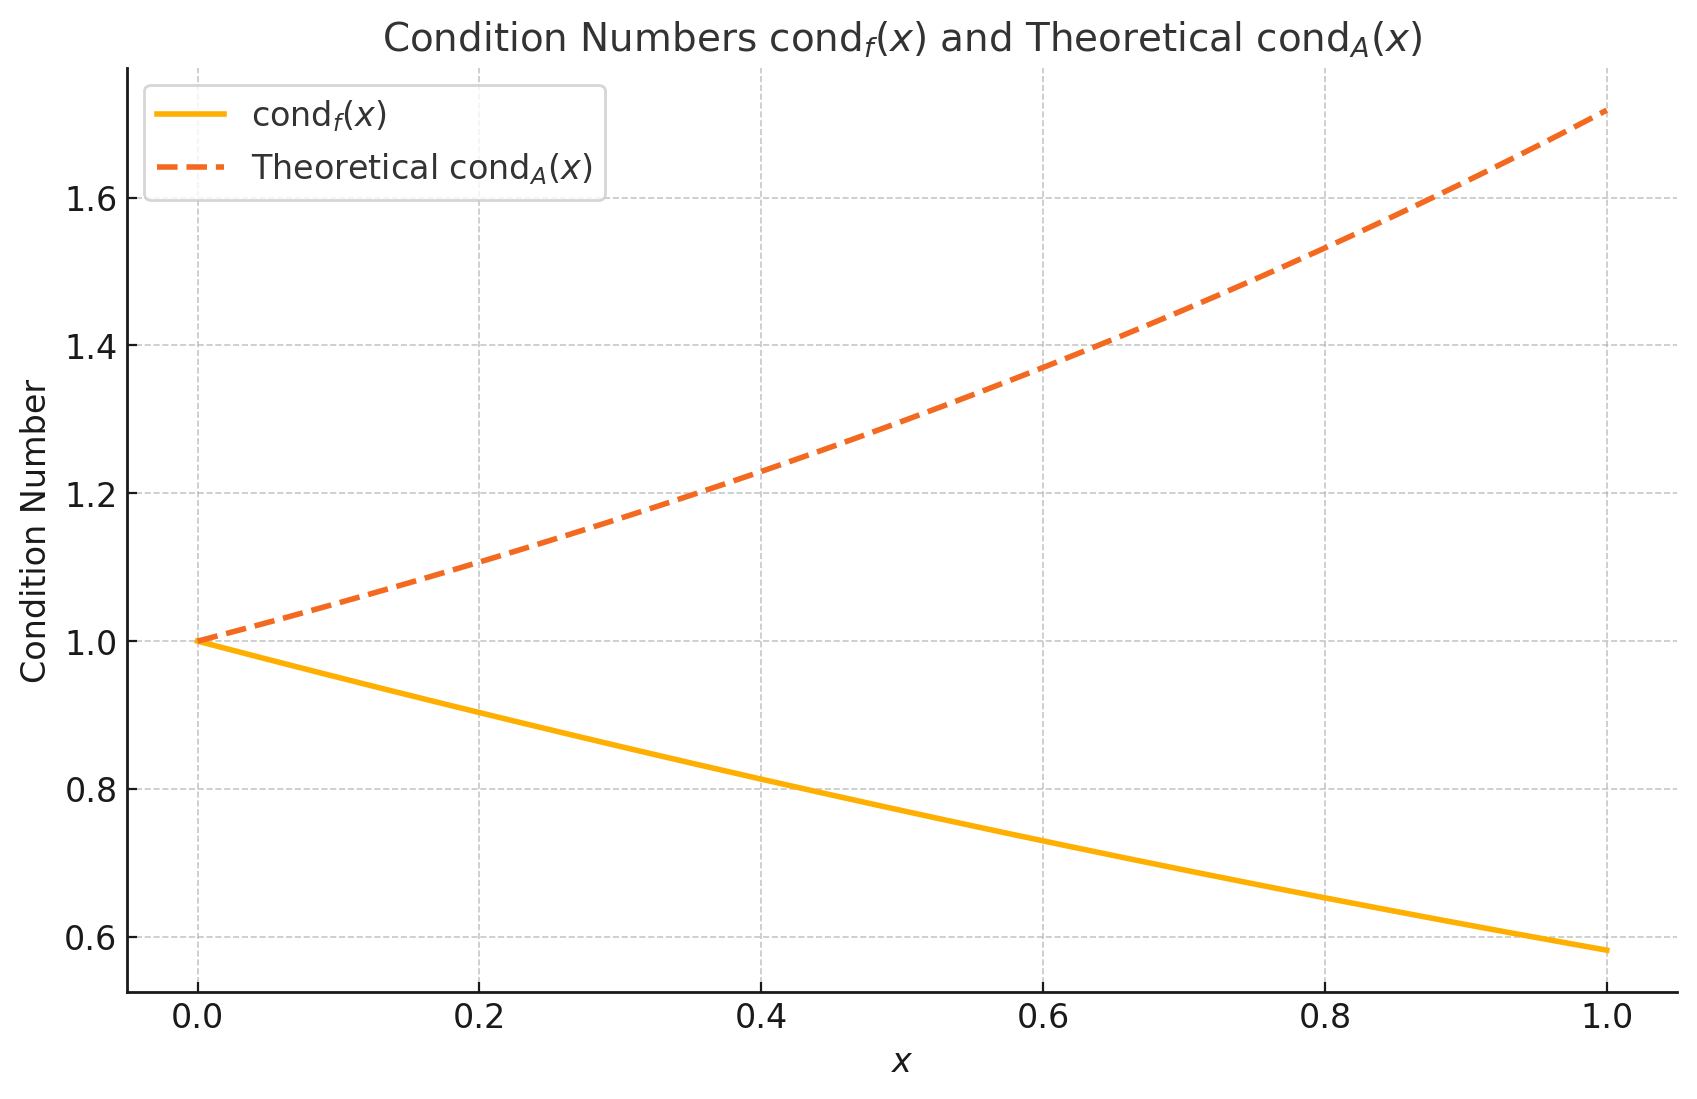
\includegraphics[width=0.6\textwidth]{1.png}
  \caption{The condition number of $f(x)$ and $A(x)$} 
  \label{fig:1}
\end{figure}

\subsection*{X. Prove lemma 4.68}
Assume the singular value of $A$ is \[0 \leq \sigma_1 \leq \sigma_2 \leq \dots \leq \sigma_n\]. Then we have 
\[\sigma_1^2 x^T x \leq x^TA^TAx\leq \sigma_n^2 x^Tx,\]
where the equality holds when $x$ is the eigenvector of $A^TA$ corresponding to $\sigma_1^2$ and $\sigma_n^2$.

So we have
\[
 \normtwo{A} = \max_{\normtwo{x} = 1} \normtwo{Ax} = \max_{\normtwo{x} = 1} \sqrt{x^TA^TAx} = \sigma_n,
 \]

And the maxium singular value of $A^{-1}$ is $\sigma_1^{-1}$, so we have
\[
  \normtwo{A^{-1}} = \sigma_1^{-1}.
\]

Therefore, we have $\text{cond}_2(A) = \frac{\sigma_n}{\sigma_1} = \frac{\sigma_{\max}}{\sigma_{\min}}$. When $A$ is normal, the singular values of $A$ is its eigenvalues, so we have $\text{cond}_2(A) = \frac{\lambda_{\max}}{\lambda_{\min}}$. And when $A$ is unitary, the singular values of $A$ are all 1, so we have $\text{cond}_2(A) = 1$.
\subsection*{XI. Wilkinson's polynomial}
We can compute the component of componentwise condition number of $f$ is\[
b_{j+1,1}(x) = \abs{\frac{a_j\frac{r^j}{\sum_{i =1}^{n}ia_ix^i-1}}{r}}=\abs{\frac{a_jr^j}{\sum_{i =1}^{n}ia_ir^i}}.
\]  
Thus The componentwise condition number of $f$ is \[
\text{cond}_{f}(x) = \sum_{j=1}^{n}b_{j}(x) = \dfrac{\sum_{i = 0}^{n-1}\abs{a_i r^i}}{\abs{\sum_{i =1}^{n}ia_ir^i}}.
\]

In the Wilkinson example, $f(x) = \prod_{k=1}^{p}(x-k)$ and $r = p$. Consider $g(x) = \prod_{k = 1}^{p} (x+k)$,
then g(x) is a polynomial with the same absolute value of coefficients as $f(x)$, and all the coefficients of $g(x)$ are positive. Thus we have \[\sum_{i = 0}^{n-1}\abs{a_i r^i} = g(r) = g(p) = \frac{(2p)!}{p!}.\]

And the denominator of the componentwise condition number of $f$ is \[\abs{\sum_{i =1}^{n}ia_ir^i} = pf'(p) =  p!.\]

Therefore, the componentwise condition number of $f$ is \[\text{cond}_{f}(x) = \frac{(2p)!}{p!p!} = \binom{2p}{p}.\]

When $p$ is big, the condition number is very large. So by the comprison, we can know that different ways of computing the condition number will lead to similar result.

\subsection*{XII. division of two FPNs}
Set $\beta = 10, p = 2, a = 5.0$ and $b = 9.9$. 

Then we have $a / b = 0.5050505……$ and $\fl(a/b) = 5.1 * 10^{-1}$ since $a/b$ is closer to 0.51 than 0.50.

But in the register with precision $2p = 4$, it can only store 0.505, so the result is $5.0 * 10^{-1}$.
\subsection*{XIII. bisection method}
A single precision floating point number has 24 bits of precision, and to obtain absolute accuracy of $10^{-6}$, we need 20 significant digits for fraction, and only 4 left for integer part. Thus only when the absolute value of root is less than 16 can we obtain the absolute accuracy of $10^{-6}$.

when the root is greater than 16, eg 128. We can not conpute the root with absolute accuracy less than $10^{-6}$.

\subsection*{XIV. Fitting curves}
Let us consider the polynomial-piece periodic cubic spline interpolation. the matrix of curving fitting is
\[\mathbf{A} =
  \begin{bmatrix}
    2 & \mu_1 &  &  & & & \lambda_1 \\
    \lambda_2 & 2 & \mu_2 &&  &  &  \\
     & \ddots & \ddots & \ddots &&  &  \\
     &  & \lambda_{i} & 2 & \mu_i & & \\
     &  &  & \ddots & \ddots & \ddots \\
     &  &  &   & \lambda_{N-1} & 2 & \mu_{N-1}\\
    \mu_N &  &   &   &  & \lambda_N & 2
    \end{bmatrix},
    \]
where $\mu_i + \lambda_i = 1.$

Consider infinity norm of $\mathbf{A}$, we have$\norminf{A} = 3$ and
\begin{align*}
  \norminf{A^{-1}} &= \sup_{x}\frac{\norminf{A^{-1}x}}{\norminf{x}}\\
  & = \sup_{y}\frac{\norminf{A^{-1}Ay}}{\norminf{Ay}}\\
& = \inf_{\norminf{y} = 1}\frac{1}{\norminf{Ay}} \leq 1.
\end{align*}
The last inequality holds since one of the components of $y$ must be 1 or -1. Let $y_i = 1$, then the $i$-th row of $Ay$ is $2 - y_{i-1} \lambda_{i} - y_{i+1} \mu_{i} \geq 1$.

Then $\text{cond} A = \norminf{A}\norminf{A^{-1}} \leq 3$

when two point are close without loss of generality, assume that $x_1$ is very closer to $x_N$, and consider the limit case where $x_1 =x_N$. Then we have $\mu_1 = \lambda_N = 0$ and $\lambda_1 = \mu_N = 1$.

let $y = (1,0,\ldots,0,-1)^T$, then we have $\norminf{Ay} = 1$ and $\norminf{A^{-1}} = 1$.

At this point, the condition number of $A$ reaches its maxium value of 3. Similarly, we can show that when two points are close, the condition number is relatively large.

\textit{remark: this problem maybe have some errors since the condition number A is bounded by 3, which is not very large. And by theorem 3.66, we can know this algorithm is well-conditioned.}

\section{Exercise}
\subsection*{Exercise 4.33}

\[
\begin{array}{|l|l|l|}
\hline
\textbf{Case 1: $b = 8.769 \times 10^4$} & \textbf{Case 2: $b = -5.678 \times 10^0$} & \textbf{Case 3: $b = -5.678 \times 10^3$} \\ \hline

(i)b \leftarrow 8.769 \times 10^4, e_c \leftarrow 4. &
(i)b \leftarrow -0.0005678 \times, e_c \leftarrow 4  &
(i)b \leftarrow -0.5678 \times 10^4, e_c \leftarrow 4. \\

(ii) 
M_c \leftarrow 1.234 + 8.769 = 10.003. &
(ii) M_c\leftarrow 1.2334322 &
(ii) M_c \leftarrow 1.234 - 0.5678 = 0.6662. \\

(iii) 
M_c \leftarrow 1.0003, e_c \leftarrow 5. & 
(iii)\text{Do nothing.}&
(iii) M_c \leftarrow 6.662, e_c \leftarrow 3. \\

(iv)
\text{Do nothing.} &
(iv)\text{Do nothing.} &
(iv)\text{Do nothing.} \\

(v) 
M_c \leftarrow 1.000. & 
(v) M_c \leftarrow 1.233&
(v) M_c \leftarrow 6.662. \\

(vi) 
c = 1.000 \times 10^5. & 
(vi)c = 1.233 \times 10^4. &
(vi)c = 6.662 \times 10^3. \\ \hline
\end{array}
\]

\subsection*{Exercise 4.42}
Set $\beta = 10$ and $p = 2$ and consider the following FPNs: $a_1 = 10, a_2 = a_3 =0.5$.
if we compute in ascending order, we have 
\begin{align*}
  a_2 + a_3 &= 1.0,\\
  a_1 + a_2 + a_3 &= 10 + 1.0 = 11.
\end{align*}
Otherwise, we have
\begin{align*}
  a_1 + a_2 &= 10,\\
  a_1 + a_2 + a_3 &= 10 +0.5 = 10.
\end{align*}
Thus the $\delta$ in first case is 0 and the $\delta$ in second case is \(-\frac{1}{11}\). So carry out addition in ascending oder is better.

\subsection*{Exercise 4.43}
\begin{align*}
  \fl(a_1b_1 + a_2b_2 + a_3b_3) &\approx (1+\delta_2) \fl(a_1b_1) + (1+\delta_2) \fl(a_2b_2) + (1+2\delta_2) \fl(a_3b_3)\\
&= (1+\delta_2)(1 + \delta_1)(a_1b_1 + a_2b_2 + a_3b_3)\\
 &= (1+\delta_3)(a_1b_1 + a_2b_2 + a_3b_3)
\end{align*}
where $(1 + \delta_2) \leq (1+\epsilon_u)^2$ and $(1+\delta_1) \leq (1+\epsilon_u)$. so $\abs{\delta_3} \leq (1+\epsilon_u)^3-1\approx3\epsilon_u$

And we can conclude that 
\[
\fl (\sum_{i = 1}^{m}\prod_{j = 1}^{n}a_{i,j}) = (1+\delta)(\sum_{i = 1}^{m}\prod_{j = 1}^{n}a_{i,j})
\]
where $\abs{\delta} \leq (1+\epsilon_i)^{n+m}-1\approx (n+m)\epsilon_u$.

\subsection*{Exercise 4.80}
Noticed that the function $f$ in this exercise is same with example 4.79, so we have \[\text{cond}_f = \frac{x}{\sin x}.\]
Futhermore, we have \[f_A(x) = \frac{(\sin x)(1+\delta_1)}{(1+(\cos x)(1+\delta_2))(1+\delta_3)}(1+\delta_4),\] where $\abs{\delta_i} \leq \epsilon_u$ for i = 1,2,3,4.
Nelect the quardratic and higher terms, the above quation is equivalent to \[f_A(x) = \frac{\sin x}{1+ \cos x} \left\{1+\delta_1-\delta_3+\delta_4-\delta_2\cos x\right\}.\]
hence we have $\varphi(x) = 3 + \cos x$ and \[\text{cond}_A(x)\leq \frac{\sin x}{x}(3+\cos x) \leq 4\]
so the algorithm is well-conditioned in this interval.

\end{document}
